\documentclass[]{article}
\usepackage{lmodern}
\usepackage{amssymb,amsmath}
\usepackage{ifxetex,ifluatex}
\usepackage{fixltx2e} % provides \textsubscript
\ifnum 0\ifxetex 1\fi\ifluatex 1\fi=0 % if pdftex
  \usepackage[T1]{fontenc}
  \usepackage[utf8]{inputenc}
\else % if luatex or xelatex
  \ifxetex
    \usepackage{mathspec}
  \else
    \usepackage{fontspec}
  \fi
  \defaultfontfeatures{Ligatures=TeX,Scale=MatchLowercase}
\fi
% use upquote if available, for straight quotes in verbatim environments
\IfFileExists{upquote.sty}{\usepackage{upquote}}{}
% use microtype if available
\IfFileExists{microtype.sty}{%
\usepackage{microtype}
\UseMicrotypeSet[protrusion]{basicmath} % disable protrusion for tt fonts
}{}
\usepackage[margin=1in]{geometry}
\usepackage{hyperref}
\hypersetup{unicode=true,
            pdfborder={0 0 0},
            breaklinks=true}
\urlstyle{same}  % don't use monospace font for urls
\usepackage{color}
\usepackage{fancyvrb}
\newcommand{\VerbBar}{|}
\newcommand{\VERB}{\Verb[commandchars=\\\{\}]}
\DefineVerbatimEnvironment{Highlighting}{Verbatim}{commandchars=\\\{\}}
% Add ',fontsize=\small' for more characters per line
\usepackage{framed}
\definecolor{shadecolor}{RGB}{248,248,248}
\newenvironment{Shaded}{\begin{snugshade}}{\end{snugshade}}
\newcommand{\AlertTok}[1]{\textcolor[rgb]{0.94,0.16,0.16}{#1}}
\newcommand{\AnnotationTok}[1]{\textcolor[rgb]{0.56,0.35,0.01}{\textbf{\textit{#1}}}}
\newcommand{\AttributeTok}[1]{\textcolor[rgb]{0.77,0.63,0.00}{#1}}
\newcommand{\BaseNTok}[1]{\textcolor[rgb]{0.00,0.00,0.81}{#1}}
\newcommand{\BuiltInTok}[1]{#1}
\newcommand{\CharTok}[1]{\textcolor[rgb]{0.31,0.60,0.02}{#1}}
\newcommand{\CommentTok}[1]{\textcolor[rgb]{0.56,0.35,0.01}{\textit{#1}}}
\newcommand{\CommentVarTok}[1]{\textcolor[rgb]{0.56,0.35,0.01}{\textbf{\textit{#1}}}}
\newcommand{\ConstantTok}[1]{\textcolor[rgb]{0.00,0.00,0.00}{#1}}
\newcommand{\ControlFlowTok}[1]{\textcolor[rgb]{0.13,0.29,0.53}{\textbf{#1}}}
\newcommand{\DataTypeTok}[1]{\textcolor[rgb]{0.13,0.29,0.53}{#1}}
\newcommand{\DecValTok}[1]{\textcolor[rgb]{0.00,0.00,0.81}{#1}}
\newcommand{\DocumentationTok}[1]{\textcolor[rgb]{0.56,0.35,0.01}{\textbf{\textit{#1}}}}
\newcommand{\ErrorTok}[1]{\textcolor[rgb]{0.64,0.00,0.00}{\textbf{#1}}}
\newcommand{\ExtensionTok}[1]{#1}
\newcommand{\FloatTok}[1]{\textcolor[rgb]{0.00,0.00,0.81}{#1}}
\newcommand{\FunctionTok}[1]{\textcolor[rgb]{0.00,0.00,0.00}{#1}}
\newcommand{\ImportTok}[1]{#1}
\newcommand{\InformationTok}[1]{\textcolor[rgb]{0.56,0.35,0.01}{\textbf{\textit{#1}}}}
\newcommand{\KeywordTok}[1]{\textcolor[rgb]{0.13,0.29,0.53}{\textbf{#1}}}
\newcommand{\NormalTok}[1]{#1}
\newcommand{\OperatorTok}[1]{\textcolor[rgb]{0.81,0.36,0.00}{\textbf{#1}}}
\newcommand{\OtherTok}[1]{\textcolor[rgb]{0.56,0.35,0.01}{#1}}
\newcommand{\PreprocessorTok}[1]{\textcolor[rgb]{0.56,0.35,0.01}{\textit{#1}}}
\newcommand{\RegionMarkerTok}[1]{#1}
\newcommand{\SpecialCharTok}[1]{\textcolor[rgb]{0.00,0.00,0.00}{#1}}
\newcommand{\SpecialStringTok}[1]{\textcolor[rgb]{0.31,0.60,0.02}{#1}}
\newcommand{\StringTok}[1]{\textcolor[rgb]{0.31,0.60,0.02}{#1}}
\newcommand{\VariableTok}[1]{\textcolor[rgb]{0.00,0.00,0.00}{#1}}
\newcommand{\VerbatimStringTok}[1]{\textcolor[rgb]{0.31,0.60,0.02}{#1}}
\newcommand{\WarningTok}[1]{\textcolor[rgb]{0.56,0.35,0.01}{\textbf{\textit{#1}}}}
\usepackage{graphicx,grffile}
\makeatletter
\def\maxwidth{\ifdim\Gin@nat@width>\linewidth\linewidth\else\Gin@nat@width\fi}
\def\maxheight{\ifdim\Gin@nat@height>\textheight\textheight\else\Gin@nat@height\fi}
\makeatother
% Scale images if necessary, so that they will not overflow the page
% margins by default, and it is still possible to overwrite the defaults
% using explicit options in \includegraphics[width, height, ...]{}
\setkeys{Gin}{width=\maxwidth,height=\maxheight,keepaspectratio}
\IfFileExists{parskip.sty}{%
\usepackage{parskip}
}{% else
\setlength{\parindent}{0pt}
\setlength{\parskip}{6pt plus 2pt minus 1pt}
}
\setlength{\emergencystretch}{3em}  % prevent overfull lines
\providecommand{\tightlist}{%
  \setlength{\itemsep}{0pt}\setlength{\parskip}{0pt}}
\setcounter{secnumdepth}{0}
% Redefines (sub)paragraphs to behave more like sections
\ifx\paragraph\undefined\else
\let\oldparagraph\paragraph
\renewcommand{\paragraph}[1]{\oldparagraph{#1}\mbox{}}
\fi
\ifx\subparagraph\undefined\else
\let\oldsubparagraph\subparagraph
\renewcommand{\subparagraph}[1]{\oldsubparagraph{#1}\mbox{}}
\fi

%%% Use protect on footnotes to avoid problems with footnotes in titles
\let\rmarkdownfootnote\footnote%
\def\footnote{\protect\rmarkdownfootnote}

%%% Change title format to be more compact
\usepackage{titling}

% Create subtitle command for use in maketitle
\providecommand{\subtitle}[1]{
  \posttitle{
    \begin{center}\large#1\end{center}
    }
}

\setlength{\droptitle}{-2em}

  \title{}
    \pretitle{\vspace{\droptitle}}
  \posttitle{}
    \author{}
    \preauthor{}\postauthor{}
    \date{}
    \predate{}\postdate{}
  
\usepackage{graphicx}				% Use pdf, png, jpg, or eps§ with pdflatex; use eps in DVI mode
\usepackage{amssymb,amsmath}
\usepackage{natbib}
\usepackage{bm}
\usepackage{xcolor}
\usepackage{tikz}
\usepackage{ctable}
% \usepackage{newtxtext} % Times-like font
% \usepackage{titlesec}
% \titleformat*{\section}{\Large\bfseries\sffamily}
% \titleformat*{\subsection}{\large\bfseries\sffamily}

%%%%%%%%%%%
% Math Macros
\newcommand{\bmA}{\ensuremath{\bm A}}
\newcommand{\bma}{\ensuremath{\bm a}}
\newcommand{\bmB}{\ensuremath{\bm B}}
\newcommand{\bmb}{\ensuremath{\bm b}}
\newcommand{\bmC}{\ensuremath{\bm C}}
\newcommand{\bmc}{\ensuremath{\bm c}}
\newcommand{\bmD}{\ensuremath{\bm D}}
\newcommand{\bmd}{\ensuremath{\bm d}}
\newcommand{\bmE}{\ensuremath{\bm E}}
\newcommand{\bme}{\ensuremath{\bm e}}
\newcommand{\bmF}{\ensuremath{\bm F}}
\newcommand{\bmG}{\ensuremath{\bm G}}
\newcommand{\bmg}{\ensuremath{\bm g}}
\newcommand{\bmH}{\ensuremath{\bm H}}
\newcommand{\bmI}{\ensuremath{\bm I}}
\newcommand{\bmJ}{\ensuremath{\bm J}}
\newcommand{\bmK}{\ensuremath{\bm K}}
\newcommand{\bmL}{\ensuremath{\bm L}}
\newcommand{\bmM}{\ensuremath{\bm M}}
\newcommand{\bmP}{\ensuremath{\bm P}}
\newcommand{\bmQ}{\ensuremath{\bm Q}}
\newcommand{\bmq}{\ensuremath{\bm q}}
\newcommand{\bmR}{\ensuremath{\bm R}}
\newcommand{\bmr}{\ensuremath{\bm r}}
\newcommand{\bmS}{\ensuremath{\bm S}}
\newcommand{\bms}{\ensuremath{\bm s}}
\newcommand{\bmT}{\ensuremath{\bm T}}
\newcommand{\bmt}{\ensuremath{\bm t}}
\newcommand{\bmU}{\ensuremath{\bm U}}
\newcommand{\bmu}{\ensuremath{\bm u}}
\newcommand{\bmV}{\ensuremath{\bm V}}
\newcommand{\bmv}{\ensuremath{\bm v}}
\newcommand{\bmW}{\ensuremath{\bm W}}
\newcommand{\bmw}{\ensuremath{\bm w}}
\newcommand{\bmX}{\ensuremath{\bm X}}
\newcommand{\bmx}{\ensuremath{\bm x}}
\newcommand{\bmY}{\ensuremath{\bm Y}}
\newcommand{\bmy}{\ensuremath{\bm y}}
\newcommand{\bmZ}{\ensuremath{\bm Z}}
\newcommand{\bmz}{\ensuremath{\bm z}}


\newcommand{\bmalpha}{\ensuremath{\bm{\alpha}}}
\newcommand{\bmbeta}{\ensuremath{\bm{\beta}}}
\newcommand{\bmdelta}{\ensuremath{\bm{\delta}}}
\newcommand{\bmeta}{\ensuremath{\bm{\eta}}}
\newcommand{\bmepsilon}{\ensuremath{\bm{\epsilon}}}
\newcommand{\bmGamma}{\ensuremath{\bm{\Gamma}}}
\newcommand{\bmgamma}{\ensuremath{\bm{\gamma}}}
\newcommand{\bmLambda}{\ensuremath{\bm{\Lambda}}}
\newcommand{\bmmu}{\ensuremath{\bm{\mu}}}
\newcommand{\bmphi}{\ensuremath{\bm{\phi}}}
\newcommand{\bmSigma}{\ensuremath{\bm{\Sigma}}}
\newcommand{\bmtheta}{\ensuremath{\bm{\theta}}}
\newcommand{\bmzeta}{\ensuremath{\bm{\zeta}}}

\newcommand{\rank}{\ensuremath{\mathsf{rank}}}
\newcommand{\nullity}{\ensuremath{\mathsf{nullity}}}
\newcommand{\trace}{\ensuremath{\mathsf{tr}}}
\newcommand{\diag}{\ensuremath{\mathsf{diag}}}
\newcommand{\vecspan}{\ensuremath{\mathsf{span}}}

\newcommand{\mT}{\ensuremath{\mathsf{T}}}

\newcommand{\bbh}{\ensuremath{\hat{\bmbeta}}}
\newcommand{\Rn}{\ensuremath{\mathbb{R}^n}}
\newcommand{\Rnp}{\ensuremath{\mathbb{R}^{n\times p}}}
\newcommand{\Pa}{\ensuremath{{\bmP}_{\bmA}}}
\newcommand{\Pb}{\ensuremath{{\bmP}_{\bmB}}}
\newcommand{\Pv}{\ensuremath{{\bmP}_\mathcal{V}}}
\newcommand{\Pw}{\ensuremath{{\bmP}_\mathcal{W}}}
\newcommand{\Px}{\ensuremath{{\bmP}_{\bmX}}}
\newcommand{\XtX}{\ensuremath{\bmX^\mT\bmX}}
\newcommand{\XtXinv}{\ensuremath{(\bmX^\mT\bmX)^{-1}}}
\newcommand{\gtb}{\ensuremath{\bmg^\mT\bmbeta}}

\DeclareMathOperator*{\argmin}{arg\,min}
\newcommand{\bbmx}{\ensuremath{\begin{bmatrix}}}
\newcommand{\ebmx}{\ensuremath{\end{bmatrix}}}

\newcommand{\E}{\ensuremath{\mathrm{E}}}
\newcommand{\Var}{\ensuremath{\mathrm{Var}}}
\newcommand{\Cov}{\ensuremath{\mathrm{Cov}}}

\newcommand{\FWER}{\ensuremath{\mathrm{FWER}}}
\newcommand{\PCER}{\ensuremath{\mathrm{PCER}}}
\newcommand{\FDR}{\ensuremath{\mathrm{FDR}}}
\newcommand{\sFWER}{\ensuremath{\mathrm{sFWER}}}
\usepackage{booktabs}
\usepackage{longtable}
\usepackage{array}
\usepackage{multirow}
\usepackage{wrapfig}
\usepackage{float}
\usepackage{colortbl}
\usepackage{pdflscape}
\usepackage{tabu}
\usepackage{threeparttable}
\usepackage{threeparttablex}
\usepackage[normalem]{ulem}
\usepackage{makecell}
\usepackage{xcolor}

\begin{document}

\hypertarget{isaacs-stuff}{%
\section{Isaac's stuff}\label{isaacs-stuff}}

\begin{center}\rule{0.5\linewidth}{\linethickness}\end{center}

\begin{center}\rule{0.5\linewidth}{\linethickness}\end{center}

\hypertarget{scraping}{%
\subsubsection{Scraping}\label{scraping}}

\begin{Shaded}
\begin{Highlighting}[]
\KeywordTok{library}\NormalTok{(dplyr)}
\end{Highlighting}
\end{Shaded}

\begin{verbatim}
## Warning: package 'dplyr' was built under R version 3.6.2
\end{verbatim}

\begin{verbatim}
## 
## Attaching package: 'dplyr'
\end{verbatim}

\begin{verbatim}
## The following objects are masked from 'package:stats':
## 
##     filter, lag
\end{verbatim}

\begin{verbatim}
## The following objects are masked from 'package:base':
## 
##     intersect, setdiff, setequal, union
\end{verbatim}

\begin{Shaded}
\begin{Highlighting}[]
\KeywordTok{library}\NormalTok{(rvest)}
\KeywordTok{library}\NormalTok{(tidyverse)}
\end{Highlighting}
\end{Shaded}

\begin{verbatim}
## Warning: package 'tidyverse' was built under R version 3.6.2
\end{verbatim}

\begin{verbatim}
## -- Attaching packages --------------------------------------- tidyverse 1.3.1 --
\end{verbatim}

\begin{verbatim}
## v ggplot2 3.3.5     v purrr   0.3.4
## v tibble  3.1.0     v stringr 1.4.0
## v tidyr   1.1.3     v forcats 0.5.1
## v readr   1.4.0
\end{verbatim}

\begin{verbatim}
## Warning: package 'ggplot2' was built under R version 3.6.2
\end{verbatim}

\begin{verbatim}
## Warning: package 'tibble' was built under R version 3.6.2
\end{verbatim}

\begin{verbatim}
## Warning: package 'tidyr' was built under R version 3.6.2
\end{verbatim}

\begin{verbatim}
## Warning: package 'readr' was built under R version 3.6.2
\end{verbatim}

\begin{verbatim}
## Warning: package 'purrr' was built under R version 3.6.2
\end{verbatim}

\begin{verbatim}
## Warning: package 'forcats' was built under R version 3.6.2
\end{verbatim}

\begin{verbatim}
## -- Conflicts ------------------------------------------ tidyverse_conflicts() --
## x dplyr::filter()         masks stats::filter()
## x readr::guess_encoding() masks rvest::guess_encoding()
## x dplyr::lag()            masks stats::lag()
\end{verbatim}

\begin{Shaded}
\begin{Highlighting}[]
\KeywordTok{library}\NormalTok{(kableExtra)}
\end{Highlighting}
\end{Shaded}

\begin{verbatim}
## Warning: package 'kableExtra' was built under R version 3.6.2
\end{verbatim}

\begin{verbatim}
## 
## Attaching package: 'kableExtra'
\end{verbatim}

\begin{verbatim}
## The following object is masked from 'package:dplyr':
## 
##     group_rows
\end{verbatim}

\begin{Shaded}
\begin{Highlighting}[]
\KeywordTok{library}\NormalTok{(ggplot2)}
\KeywordTok{library}\NormalTok{(reshape2)}
\end{Highlighting}
\end{Shaded}

\begin{verbatim}
## 
## Attaching package: 'reshape2'
\end{verbatim}

\begin{verbatim}
## The following object is masked from 'package:tidyr':
## 
##     smiths
\end{verbatim}

\hypertarget{wnba-scraping}{%
\subsection{wnba scraping}\label{wnba-scraping}}

\begin{Shaded}
\begin{Highlighting}[]
\NormalTok{wilson <-}\StringTok{ 'https://www.basketball-reference.com/wnba/players/w/wilsoa01w/gamelog/2022/'}
\NormalTok{wil_doc <-}\StringTok{ }\NormalTok{rvest}\OperatorTok{::}\KeywordTok{read_html}\NormalTok{(wilson)}

\NormalTok{wil_doc }\OperatorTok
\StringTok{  }\NormalTok{rvest}\OperatorTok{::}\KeywordTok{html_elements}\NormalTok{(., }\DataTypeTok{xpath =} \StringTok{"//*[(@id = 'div_wnba_pgl_basic')]"}\NormalTok{) }\OperatorTok
\StringTok{  }\NormalTok{rvest}\OperatorTok{::}\KeywordTok{html_table}\NormalTok{() ->}\StringTok{ }\NormalTok{wil}
\NormalTok{wil <-}\StringTok{ }\NormalTok{wil[[}\DecValTok{1}\NormalTok{]]}
\KeywordTok{head}\NormalTok{(wil)}
\end{Highlighting}
\end{Shaded}

\begin{verbatim}
## # A tibble: 6 x 28
##   Rk    Date   Age   Tm    ``    Opp   ``    GS    MP    FG    FGA   `FG%` `3P` 
##   <chr> <chr>  <chr> <chr> <chr> <chr> <chr> <chr> <chr> <chr> <chr> <chr> <chr>
## 1 1     2022-~ 25-2~ LVA   "@"   PHO   W (+~ 1     28:35 5     8     .625  0    
## 2 2     2022-~ 25-2~ LVA   ""    SEA   W (+~ 1     35:06 8     14    .571  1    
## 3 3     2022-~ 25-2~ LVA   "@"   WAS   L (-~ 1     29:56 4     11    .364  0    
## 4 4     2022-~ 25-2~ LVA   "@"   ATL   W (+~ 1     29:08 6     11    .545  0    
## 5 5     2022-~ 25-2~ LVA   ""    PHO   W (+~ 1     33:45 4     8     .500  0    
## 6 6     2022-~ 25-2~ LVA   ""    MIN   W (+~ 1     31:16 5     9     .556  1    
## # ... with 15 more variables: 3PA <chr>, 3P% <chr>, FT <chr>, FTA <chr>,
## #   FT% <chr>, ORB <chr>, DRB <chr>, TRB <chr>, AST <chr>, STL <chr>,
## #   BLK <chr>, TOV <chr>, PF <chr>, PTS <chr>, GmSc <chr>
\end{verbatim}

\begin{Shaded}
\begin{Highlighting}[]
\CommentTok{#wil2 <- mutate_all(wil, function(x) as.numeric(as.character(x)))}
\CommentTok{#mean(wil2['PTS'])}

\CommentTok{#wil$eFG<- (wil['FG'] + (0.5*wil['3P']))/wil['FGA']}
\CommentTok{#wil$eFG ![Screenshot]('~/Google Drive/My Drive/Sports Analytics/SportsAnalyticsBook/images/scraping1')}
\end{Highlighting}
\end{Shaded}

\begin{center}\rule{0.5\linewidth}{\linethickness}\end{center}

\hypertarget{edaprobability}{%
\subsubsection{EDA/Probability}\label{edaprobability}}

\begin{center}\rule{0.5\linewidth}{\linethickness}\end{center}

\hypertarget{baseball}{%
\subsubsection{Baseball}\label{baseball}}

\hypertarget{war-comparison-prob}{%
\paragraph{WAR comparison (Prob)}\label{war-comparison-prob}}

Link to WAR explaination:
\url{https://www.mlb.com/glossary/advanced-stats/wins-above-replacement}

Player X has a projected mean WAR of 3 with standard deviation of 2 and
player Y has a projected mean WAR of 1.5 with a standard deviation of 3.
Assume projected WAR is normally distributed. Q: What is the probability
that Player X outperforms Player Y? A: We want Pr(X\textgreater{}Y) or
Pr(X-Y\textgreater{}0).\\
Let Z = X-Y.\\
E{[}Z{]}=1.5 Var(Z)=5 Pr(Z\textgreater{}0)=1-Pr(Z \(\leq\) 0)

\begin{Shaded}
\begin{Highlighting}[]
\CommentTok{#Calculate probability Z<=0}
\NormalTok{pr <-}\StringTok{ }\KeywordTok{pnorm}\NormalTok{(}\DecValTok{0}\NormalTok{,}\FloatTok{1.5}\NormalTok{,}\KeywordTok{sqrt}\NormalTok{(}\DecValTok{5}\NormalTok{))}
\KeywordTok{print}\NormalTok{(}\DecValTok{1}\OperatorTok{-}\NormalTok{pr)}
\end{Highlighting}
\end{Shaded}

\begin{verbatim}
## [1] 0.7488325
\end{verbatim}

The Probability that Player X outperforms Player Y is 0.7488.

\hypertarget{injured-baserunner-prob}{%
\paragraph{Injured Baserunner (Prob)}\label{injured-baserunner-prob}}

A runner on first base with 2 out and nobody else on base will attempt
to steal second base on the first pitch 70\% of the time if he is fully
healthy but only 10\% of the time if he is playing through an injury.
Assume that 80\% of the player population is healthy. You see a randomly
selected runner not attempt a steal in this situation. Q: What is the
probability that the runner is playing through an injury? A: From Bayes
Theorem:

Pr(Injury given No Steal) = Pr(No Steal given Injury)*Pr(Injury)/P(No
Steal).

Pr(No Steal given Injury) = 1 - Pr(Steal given Injury) = 0.9.

Pr(Injury) = 1- Pr(Healthy) = 0.2.

Pr(No Steal) = Pr(No Steal given Injury)*Pr(Injury)+Pr(No Steal given
Healthy)*Pr(Healthy).

Pr(No Steal) = 0.9*0.2+0.7*0.8 = 0.74.

Therefore Pr(Injury given No Steal) = 0.9*0.2/0.74 = 0.243.

\hypertarget{ops-eda}{%
\paragraph{OPS (EDA)}\label{ops-eda}}

Q: Using the dataset, plot the leagues average OPS from every year in
the data to see the progression. A:

\begin{Shaded}
\begin{Highlighting}[]
\NormalTok{mlb =}\StringTok{ }\KeywordTok{read.csv}\NormalTok{(}\StringTok{'~/Google Drive/My Drive/Sports Analytics/SportsAnalyticsBook/data/mlb_team_stats_history.csv'}\NormalTok{)}
\KeywordTok{head}\NormalTok{(mlb)}
\end{Highlighting}
\end{Shaded}

\begin{verbatim}
##   yearID lgID teamID franchID divID Rank   G Ghome  W  L DivWin WCWin LgWin
## 1   1976   NL    ATL      ATL     W    6 162    81 70 92      N           N
## 2   1976   AL    BAL      BAL     E    2 162    81 88 74      N           N
## 3   1976   AL    BOS      BOS     E    3 162    81 83 79      N           N
## 4   1976   AL    CAL      ANA     W    4 162    81 76 86      N           N
## 5   1976   AL    CHA      CHW     W    6 161    80 64 97      N           N
## 6   1976   NL    CHN      CHC     E    4 162    81 75 87      N           N
##   WSWin   R   AB    H  X1B X2B X3B  HR  BB  SO  SB CS HBP SF  RA    BA  ER  ERA
## 1     N 620 5345 1309 1027 170  30  82 589 811  74 61  19 47 700 0.245 617 3.86
## 2     N 619 5457 1326  966 213  28 119 519 883 150 61  23 35 598 0.243 541 3.32
## 3     N 716 5511 1448 1004 257  53 134 500 832  95 70  29 59 660 0.263 571 3.52
## 4     N 550 5385 1265  969 210  23  63 534 812 126 80  42 48 631 0.235 551 3.36
## 5     N 586 5532 1410 1082 209  46  73 471 739 120 53  34 55 745 0.255 684 4.25
## 6     N 611 5519 1386 1041 216  24 105 490 834  74 74  30 41 728 0.251 643 3.93
##   CG SHO SV IPouts   HA HRA BBA SOA   E  DP    FP              name
## 1 33  13 27   4314 1435  86 564 818 167 151 0.973    Atlanta Braves
## 2 59  16 23   4406 1396  80 489 678 118 157 0.982 Baltimore Orioles
## 3 49  13 27   4374 1495 109 409 673 141 148 0.978    Boston Red Sox
## 4 64  15 17   4432 1323  95 553 992 150 139 0.977 California Angels
## 5 54  10 22   4344 1460  87 600 802 130 155 0.979 Chicago White Sox
## 6 27  12 33   4414 1511 123 490 850 140 145 0.978      Chicago Cubs
##                            park attendance BPF PPF teamIDBR teamIDlahman45
## 1 Atlanta-Fulton County Stadium     818179 106 108      ATL            ATL
## 2              Memorial Stadium    1058609  94  93      BAL            BAL
## 3                Fenway Park II    1895846 113 112      BOS            BOS
## 4               Anaheim Stadium    1006774  93  94      CAL            CAL
## 5                 Comiskey Park     914945 101 102      CHW            CHA
## 6                 Wrigley Field    1026217 108 109      CHC            CHN
##   teamIDretro
## 1         ATL
## 2         BAL
## 3         BOS
## 4         CAL
## 5         CHA
## 6         CHN
\end{verbatim}

\begin{Shaded}
\begin{Highlighting}[]
\CommentTok{# make new variables}
\NormalTok{mlb=}\KeywordTok{mutate}\NormalTok{(mlb,}\DataTypeTok{SLG=}\NormalTok{(X1B}\OperatorTok{+}\DecValTok{2}\OperatorTok{*}\NormalTok{X2B}\OperatorTok{+}\DecValTok{3}\OperatorTok{*}\NormalTok{X3B}\OperatorTok{+}\DecValTok{4}\OperatorTok{*}\NormalTok{HR)}\OperatorTok{/}\NormalTok{(AB))}
\NormalTok{mlb=}\KeywordTok{mutate}\NormalTok{(mlb,}\DataTypeTok{OBP=}\NormalTok{(H}\OperatorTok{+}\NormalTok{BB}\OperatorTok{+}\NormalTok{HBP)}\OperatorTok{/}\NormalTok{(AB}\OperatorTok{+}\NormalTok{BB}\OperatorTok{+}\NormalTok{HBP}\OperatorTok{+}\NormalTok{SF))}
\NormalTok{mlb=}\KeywordTok{mutate}\NormalTok{(mlb,}\DataTypeTok{OPS=}\NormalTok{OBP}\OperatorTok{+}\NormalTok{SLG)}

\CommentTok{# get avg ops}
\KeywordTok{summarize}\NormalTok{(mlb, }\DataTypeTok{Average =} \KeywordTok{mean}\NormalTok{(OPS,}\DataTypeTok{na.rm=}\NormalTok{T))}
\end{Highlighting}
\end{Shaded}

\begin{verbatim}
##     Average
## 1 0.7330384
\end{verbatim}

\begin{Shaded}
\begin{Highlighting}[]
\CommentTok{# get avg ops by year}
\KeywordTok{group_by}\NormalTok{(mlb, yearID)}\OperatorTok
\KeywordTok{summarize}\NormalTok{(}\DataTypeTok{Average =} \KeywordTok{mean}\NormalTok{(OPS, }\DataTypeTok{na.rm=}\NormalTok{T))}
\end{Highlighting}
\end{Shaded}

\begin{verbatim}
## # A tibble: 43 x 2
##    yearID Average
##     <int>   <dbl>
##  1   1976   0.681
##  2   1977   0.730
##  3   1978   0.702
##  4   1979   0.727
##  5   1980   0.714
##  6   1981   0.688
##  7   1982   0.712
##  8   1983   0.714
##  9   1984   0.707
## 10   1985   0.714
## # ... with 33 more rows
\end{verbatim}

\begin{Shaded}
\begin{Highlighting}[]
\KeywordTok{group_by}\NormalTok{(mlb, yearID)}\OperatorTok
\KeywordTok{summarize}\NormalTok{(}\DataTypeTok{Average =} \KeywordTok{mean}\NormalTok{(OPS, }\DataTypeTok{na.rm=}\NormalTok{T))}\OperatorTok\NormalTok{View}

\CommentTok{#create new dataset}
\NormalTok{mlbYr=}\KeywordTok{group_by}\NormalTok{(mlb, yearID)}\OperatorTok
\KeywordTok{summarize}\NormalTok{(}\DataTypeTok{Average =} \KeywordTok{mean}\NormalTok{(OPS, }\DataTypeTok{na.rm=}\NormalTok{T))}

\CommentTok{#plot it}
\KeywordTok{ggplot}\NormalTok{(mlbYr, }\KeywordTok{aes}\NormalTok{(}\DataTypeTok{x=}\NormalTok{yearID, }\DataTypeTok{y=}\NormalTok{ Average))}\OperatorTok{+}\KeywordTok{geom_point}\NormalTok{()}
\end{Highlighting}
\end{Shaded}

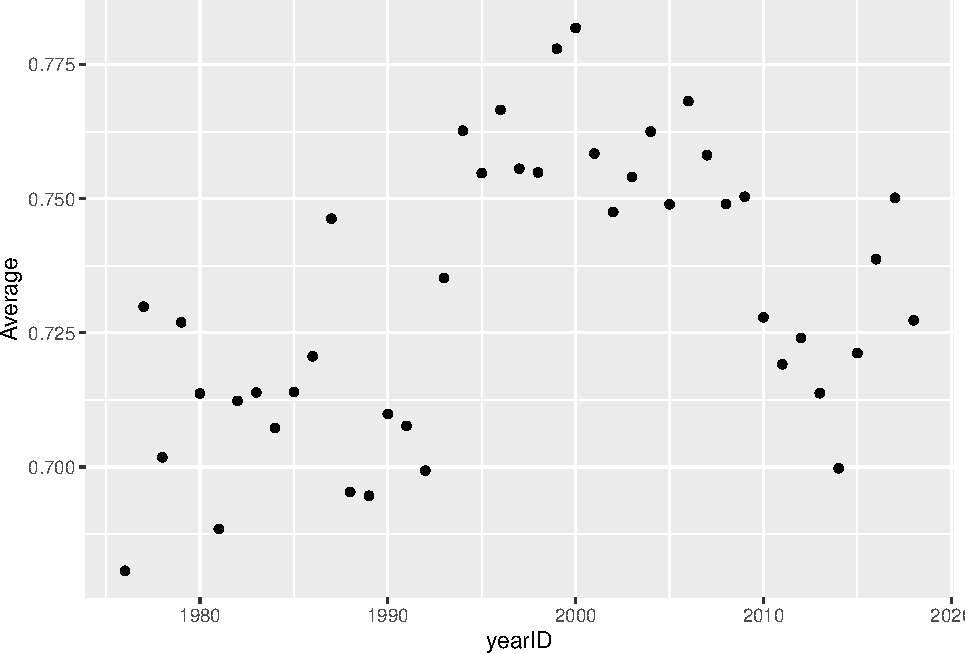
\includegraphics{22-isaac_files/figure-latex/unnamed-chunk-4-1.pdf}
Followup Q: What would cause the data to peak around the year 2000? A:
PED's

\hypertarget{run-variance-probability}{%
\paragraph{Run Variance (Probability)}\label{run-variance-probability}}

\begin{center}
\begin{tabular}{ c c c c c }
 Runs Scored & Probability \\ 
 0 & 0.55 \\  
 1 & 0.25 \\
 2 & 0.15 \\
 3 & 0.05
\end{tabular}
\end{center}

Q: Using the probability table provided, calculate the variance for runs
scored in an inning A: \(E(X)=1*0.25+2*0.15+3*0.05=0.7\)\\
\(E(X^2)=1*0.25+4*0.15+9*0.05=1.3\)\\
\(Var(X)=E(X^2)-E(X)=1.3-0.7=0.6\)

\begin{center}\rule{0.5\linewidth}{\linethickness}\end{center}

\hypertarget{tennis}{%
\subsubsection{Tennis}\label{tennis}}

Link for brief explanation of tennis scoring:
\url{https://www.sportingnews.com/us/tennis/news/tennis-scoring-explained-rules-system-points-terms/7uzp2evdhbd11obdd59p3p1cx}

\hypertarget{probability-of-winning-a-game-prob}{%
\paragraph{Probability of Winning a Game
(Prob)}\label{probability-of-winning-a-game-prob}}

The formula for the probability of a tennis player winning a game (from
Analyzing Wimbledon) is given by
\(\frac{p^4*(-8*p^3+28*p^2-34*p+15)}{p^2+(1-p)^2}\) where \(p\) is the
probability of a player winning their service point. Q: If a player wins
their service points 62\% of the time, what is the probability they win
the game? A:

\begin{Shaded}
\begin{Highlighting}[]
\NormalTok{p <-}\StringTok{ }\FloatTok{0.62}
\NormalTok{pr_game <-}\StringTok{ }\NormalTok{(p}\OperatorTok{^}\DecValTok{4}\OperatorTok{*}\NormalTok{(}\OperatorTok{-}\DecValTok{8}\OperatorTok{*}\NormalTok{p}\OperatorTok{^}\DecValTok{3}\OperatorTok{+}\DecValTok{28}\OperatorTok{*}\NormalTok{p}\OperatorTok{^}\DecValTok{2-34}\OperatorTok{*}\NormalTok{p}\OperatorTok{+}\DecValTok{15}\NormalTok{))}\OperatorTok{/}\NormalTok{(p}\OperatorTok{^}\DecValTok{2}\OperatorTok{+}\NormalTok{(}\DecValTok{1}\OperatorTok{-}\NormalTok{p)}\OperatorTok{^}\DecValTok{2}\NormalTok{)}
\NormalTok{pr_game}
\end{Highlighting}
\end{Shaded}

\begin{verbatim}
## [1] 0.7758627
\end{verbatim}

\hypertarget{graph-example-of-probability-of-winning-point-vs-probability-of-winning-game-prob}{%
\paragraph{Graph Example of Probability of Winning Point vs Probability
of Winning Game
(Prob)}\label{graph-example-of-probability-of-winning-point-vs-probability-of-winning-game-prob}}

\begin{Shaded}
\begin{Highlighting}[]
\NormalTok{game <-}\StringTok{ }\KeywordTok{c}\NormalTok{(}\DecValTok{0}\NormalTok{)}
\NormalTok{pr <-}\StringTok{ }\DecValTok{1}\OperatorTok{:}\DecValTok{100}
\ControlFlowTok{for}\NormalTok{(x }\ControlFlowTok{in}\NormalTok{ pr) \{}
\NormalTok{  p <-}\StringTok{ }\NormalTok{pr}\OperatorTok{/}\DecValTok{100}
\NormalTok{  pr_game <-}\StringTok{ }\NormalTok{(p}\OperatorTok{^}\DecValTok{4}\OperatorTok{*}\NormalTok{(}\OperatorTok{-}\DecValTok{8}\OperatorTok{*}\NormalTok{p}\OperatorTok{^}\DecValTok{3}\OperatorTok{+}\DecValTok{28}\OperatorTok{*}\NormalTok{p}\OperatorTok{^}\DecValTok{2-34}\OperatorTok{*}\NormalTok{p}\OperatorTok{+}\DecValTok{15}\NormalTok{))}\OperatorTok{/}\NormalTok{(p}\OperatorTok{^}\DecValTok{2}\OperatorTok{+}\NormalTok{(}\DecValTok{1}\OperatorTok{-}\NormalTok{p)}\OperatorTok{^}\DecValTok{2}\NormalTok{)}
\NormalTok{  game <-}\StringTok{ }\KeywordTok{c}\NormalTok{(game,pr_game)}
\NormalTok{\}}
\NormalTok{game[}\DecValTok{1}\NormalTok{]}
\end{Highlighting}
\end{Shaded}

\begin{verbatim}
## [1] 0
\end{verbatim}

\begin{Shaded}
\begin{Highlighting}[]
\NormalTok{game <-}\StringTok{ }\NormalTok{game[}\DecValTok{2}\OperatorTok{:}\DecValTok{101}\NormalTok{]}
\NormalTok{game[}\DecValTok{1}\NormalTok{]}
\end{Highlighting}
\end{Shaded}

\begin{verbatim}
## [1] 1.495898e-07
\end{verbatim}

\begin{Shaded}
\begin{Highlighting}[]
\NormalTok{df <-}\StringTok{ }\KeywordTok{do.call}\NormalTok{(rbind, }\KeywordTok{Map}\NormalTok{(data.frame, }\DataTypeTok{point_pr=}\NormalTok{pr, }\DataTypeTok{game_pr=}\NormalTok{game))}
\KeywordTok{ggplot}\NormalTok{(df, }\KeywordTok{aes}\NormalTok{(}\DataTypeTok{x=}\NormalTok{point_pr, }\DataTypeTok{y=}\NormalTok{game_pr)) }\OperatorTok{+}
\StringTok{  }\KeywordTok{geom_point}\NormalTok{()}\OperatorTok{+}\KeywordTok{xlab}\NormalTok{(}\StringTok{'Probability of Winning a Service Point'}\NormalTok{)}\OperatorTok{+}\KeywordTok{ylab}\NormalTok{(}\StringTok{'Probability of Winning a Game'}\NormalTok{)}
\end{Highlighting}
\end{Shaded}

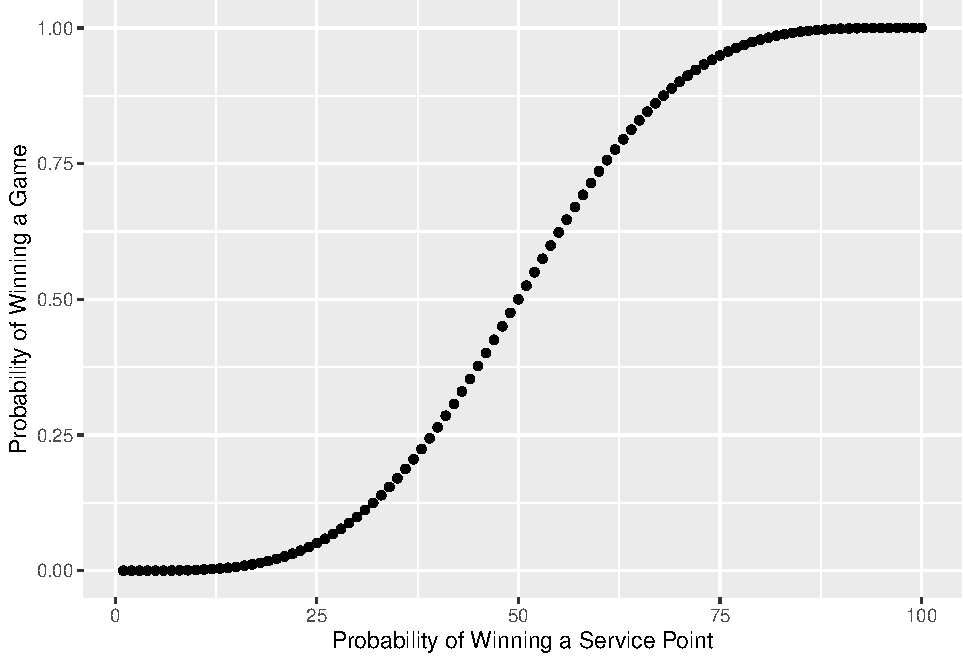
\includegraphics{22-isaac_files/figure-latex/unnamed-chunk-6-1.pdf}

\hypertarget{wnba-scores-eda}{%
\subsubsection{WNBA Scores (EDA)}\label{wnba-scores-eda}}

Q: What is the difference in PPG for a winning team at home vs a winning
team away? A:

\begin{Shaded}
\begin{Highlighting}[]
\NormalTok{wnba=}\KeywordTok{read.csv}\NormalTok{(}\StringTok{'~/Google Drive/My Drive/Sports Analytics/SportsAnalyticsBook/data/WNBA_Games2019_Scores.csv'}\NormalTok{)}
\KeywordTok{head}\NormalTok{(wnba)}
\end{Highlighting}
\end{Shaded}

\begin{verbatim}
##   Game         HomeTeam           AwayTeam Winner PTSwin PTSlose
## 1    1    Atlanta Dream       Dallas Wings   Home     76      72
## 2    2 New York Liberty      Indiana Fever   Away     81      80
## 3    3  Connecticut Sun Washington Mystics   Home     84      69
## 4    4   Minnesota Lynx        Chicago Sky   Home     89      71
## 5    5    Seattle Storm    Phoenix Mercury   Home     77      68
## 6    6   Las Vegas Aces Los Angeles Sparks   Home     83      70
##       WinningTeam
## 1   Atlanta Dream
## 2   Indiana Fever
## 3 Connecticut Sun
## 4  Minnesota Lynx
## 5   Seattle Storm
## 6  Las Vegas Aces
\end{verbatim}

\begin{Shaded}
\begin{Highlighting}[]
\KeywordTok{group_by}\NormalTok{(wnba, Winner)}\OperatorTok
\StringTok{  }\KeywordTok{summarize}\NormalTok{(}\DataTypeTok{Count=}\KeywordTok{n}\NormalTok{())}\OperatorTok
\StringTok{  }\KeywordTok{mutate}\NormalTok{(}\DataTypeTok{Percent=}\NormalTok{Count}\OperatorTok{/}\KeywordTok{sum}\NormalTok{(Count))}
\end{Highlighting}
\end{Shaded}

\begin{verbatim}
## # A tibble: 2 x 3
##   Winner Count Percent
##   <fct>  <int>   <dbl>
## 1 Away      80   0.392
## 2 Home     124   0.608
\end{verbatim}

\begin{Shaded}
\begin{Highlighting}[]
\KeywordTok{group_by}\NormalTok{(wnba, Winner)}\OperatorTok
\StringTok{  }\KeywordTok{summarize}\NormalTok{(}\DataTypeTok{Average=}\KeywordTok{mean}\NormalTok{(PTSwin,}\DataTypeTok{na.rm=}\NormalTok{T),}\DataTypeTok{sd=}\KeywordTok{sd}\NormalTok{(PTSwin,}\DataTypeTok{na.rm=}\NormalTok{T))}
\end{Highlighting}
\end{Shaded}

\begin{verbatim}
## # A tibble: 2 x 3
##   Winner Average    sd
##   <fct>    <dbl> <dbl>
## 1 Away      83.8  9.20
## 2 Home      84.8 10.8
\end{verbatim}

\begin{Shaded}
\begin{Highlighting}[]
\FloatTok{84.822-83.787}
\end{Highlighting}
\end{Shaded}

\begin{verbatim}
## [1] 1.035
\end{verbatim}

A home team winner scores on average 1.035 PPG more than an away team
winner.

\hypertarget{nfl}{%
\subsubsection{NFL}\label{nfl}}

\begin{Shaded}
\begin{Highlighting}[]
\NormalTok{nfl=}\KeywordTok{read.csv}\NormalTok{(}\StringTok{'~/Google Drive/My Drive/Sports Analytics/SportsAnalyticsBook/data/nfl_pbp.csv'}\NormalTok{)}
\NormalTok{nfl2 <-}\StringTok{ }\KeywordTok{select}\NormalTok{(nfl, }\KeywordTok{c}\NormalTok{(}\StringTok{'Date'}\NormalTok{,}\StringTok{'GameID'}\NormalTok{,}\StringTok{'qtr'}\NormalTok{,}\StringTok{'down'}\NormalTok{,}\StringTok{'time'}\NormalTok{,}\StringTok{'yrdline100'}\NormalTok{,}\StringTok{'ydstogo'}\NormalTok{,}\StringTok{'Yards.Gained'}\NormalTok{,}\StringTok{'Touchdown'}\NormalTok{,}\StringTok{'PlayType'}\NormalTok{,}\StringTok{'FieldGoalResult'}\NormalTok{,}\StringTok{'FieldGoalDistance'}\NormalTok{,}\StringTok{'ScoreDiff'}\NormalTok{,}\StringTok{'Season'}\NormalTok{))}
\KeywordTok{head}\NormalTok{(nfl2)}
\end{Highlighting}
\end{Shaded}

\begin{verbatim}
##         Date     GameID qtr down  time yrdline100 ydstogo Yards.Gained
## 1 2009-09-10 2009091000   1   NA 15:00         30       0           39
## 2 2009-09-10 2009091000   1    1 14:53         58      10            5
## 3 2009-09-10 2009091000   1    2 14:16         53       5           -3
## 4 2009-09-10 2009091000   1    3 13:35         56       8            0
## 5 2009-09-10 2009091000   1    4 13:27         56       8            0
## 6 2009-09-10 2009091000   1    1 13:16         98      10            0
##   Touchdown PlayType FieldGoalResult FieldGoalDistance ScoreDiff Season
## 1         0  Kickoff            <NA>                NA         0   2009
## 2         0     Pass            <NA>                NA         0   2009
## 3         0      Run            <NA>                NA         0   2009
## 4         0     Pass            <NA>                NA         0   2009
## 5         0     Punt            <NA>                NA         0   2009
## 6         0      Run            <NA>                NA         0   2009
\end{verbatim}

\hypertarget{th-down-analysis-eda}{%
\paragraph{4th Down Analysis (EDA)}\label{th-down-analysis-eda}}

Q: Using NFL Play by Play data, what percentage of the time do coaches
choose to go for it on 4th down? And what percentage of 4th down
attempts are successful? A:

\begin{Shaded}
\begin{Highlighting}[]
\CommentTok{# add indicator column for successful first down attempt}
\NormalTok{nfl2 <-}\StringTok{ }\NormalTok{nfl2 }\OperatorTok
\StringTok{  }\KeywordTok{mutate}\NormalTok{(}\DataTypeTok{FirstDown =} \KeywordTok{case_when}\NormalTok{(}
\NormalTok{    ydstogo }\OperatorTok{<}\StringTok{ }\NormalTok{Yards.Gained }\OperatorTok{~}\StringTok{ }\DecValTok{1}\NormalTok{,}
\NormalTok{    ydstogo }\OperatorTok{>}\StringTok{ }\NormalTok{Yards.Gained }\OperatorTok{~}\StringTok{ }\DecValTok{0}
\NormalTok{    ))}
\CommentTok{# filter by only plays on 4th down}
\NormalTok{down4 =}\StringTok{ }\KeywordTok{filter}\NormalTok{(nfl2, nfl2[}\StringTok{'down'}\NormalTok{]}\OperatorTok{==}\DecValTok{4}\NormalTok{)}

\CommentTok{#see what play types are run on fourth down and remove the noise}
\KeywordTok{group_by}\NormalTok{(down4,PlayType) }\OperatorTok
\StringTok{  }\KeywordTok{summarize}\NormalTok{(}\DataTypeTok{Count=}\KeywordTok{n}\NormalTok{())}\OperatorTok
\StringTok{  }\KeywordTok{mutate}\NormalTok{(}\DataTypeTok{Percentage=}\NormalTok{Count}\OperatorTok{/}\KeywordTok{sum}\NormalTok{(Count))}
\end{Highlighting}
\end{Shaded}

\begin{verbatim}
## # A tibble: 8 x 3
##   PlayType   Count Percentage
##   <fct>      <int>      <dbl>
## 1 Field Goal  7265  0.226    
## 2 No Play     1433  0.0446   
## 3 Pass        2239  0.0698   
## 4 Punt       19551  0.609    
## 5 QB Kneel      22  0.000685 
## 6 Run         1424  0.0444   
## 7 Sack         164  0.00511  
## 8 Timeout        1  0.0000312
\end{verbatim}

\begin{Shaded}
\begin{Highlighting}[]
\NormalTok{down4 =}\StringTok{ }\KeywordTok{filter}\NormalTok{(down4, down4[}\StringTok{'PlayType'}\NormalTok{]}\OperatorTok{!=}\StringTok{'No Play'} \OperatorTok{||}\StringTok{ }\NormalTok{down4[}\StringTok{'PlayType'}\NormalTok{]}\OperatorTok{!=}\StringTok{ 'QB Kneel'} \OperatorTok{||}\StringTok{ }\NormalTok{down4[}\StringTok{'PlayType'}\NormalTok{]}\OperatorTok{!=}\StringTok{ 'Timeout'}\NormalTok{)}

\CommentTok{# add indicator column for going for it on 4th}
\NormalTok{down4 <-}\StringTok{ }\NormalTok{down4 }\OperatorTok\StringTok{ }
\StringTok{  }\KeywordTok{mutate}\NormalTok{(}\DataTypeTok{GoForIt =} \KeywordTok{case_when}\NormalTok{(}
\NormalTok{    PlayType }\OperatorTok{==}\StringTok{ 'Pass'} \OperatorTok{~}\StringTok{ }\DecValTok{1}\NormalTok{,}
\NormalTok{    PlayType }\OperatorTok{==}\StringTok{ 'Run'} \OperatorTok{~}\StringTok{ }\DecValTok{1}\NormalTok{,}
\NormalTok{    PlayType }\OperatorTok{==}\StringTok{ 'Sack'} \OperatorTok{~}\StringTok{ }\DecValTok{1}\NormalTok{,}
\NormalTok{    PlayType }\OperatorTok{==}\StringTok{ 'Field Goal'} \OperatorTok{~}\StringTok{ }\DecValTok{0}\NormalTok{, }
\NormalTok{    PlayType }\OperatorTok{==}\StringTok{ 'Punt'} \OperatorTok{~}\StringTok{ }\DecValTok{0}
\NormalTok{  ))}
\CommentTok{# get percentage of 4th downs are gone for}
\KeywordTok{group_by}\NormalTok{(down4,GoForIt) }\OperatorTok
\StringTok{  }\KeywordTok{summarize}\NormalTok{(}\DataTypeTok{Count=}\KeywordTok{n}\NormalTok{())}\OperatorTok
\StringTok{  }\KeywordTok{mutate}\NormalTok{(}\DataTypeTok{Percentage=}\NormalTok{Count}\OperatorTok{/}\KeywordTok{sum}\NormalTok{(Count))}
\end{Highlighting}
\end{Shaded}

\begin{verbatim}
## # A tibble: 3 x 3
##   GoForIt Count Percentage
##     <dbl> <int>      <dbl>
## 1       0 26816     0.835 
## 2       1  3827     0.119 
## 3      NA  1456     0.0454
\end{verbatim}

\begin{Shaded}
\begin{Highlighting}[]
\CommentTok{# get percentage of successful attempted 4th downs }
\NormalTok{down4 }\OperatorTok
\StringTok{  }\KeywordTok{filter}\NormalTok{(down4[}\StringTok{'GoForIt'}\NormalTok{]}\OperatorTok{==}\DecValTok{1}\NormalTok{) }\OperatorTok
\StringTok{  }\KeywordTok{group_by}\NormalTok{(FirstDown) }\OperatorTok
\StringTok{    }\KeywordTok{summarize}\NormalTok{(}\DataTypeTok{Count=}\KeywordTok{n}\NormalTok{())}\OperatorTok
\StringTok{    }\KeywordTok{mutate}\NormalTok{(}\DataTypeTok{Percentage=}\NormalTok{Count}\OperatorTok{/}\KeywordTok{sum}\NormalTok{(Count))  }
\end{Highlighting}
\end{Shaded}

\begin{verbatim}
## # A tibble: 3 x 3
##   FirstDown Count Percentage
##       <dbl> <int>      <dbl>
## 1         0  1971     0.515 
## 2         1  1553     0.406 
## 3        NA   303     0.0792
\end{verbatim}

11\% of 4th downs are gone for and 40\% of those are successful,
regardless of how many yards to go there are

\hypertarget{probability-of-outcome-based-on-field-position-graph}{%
\paragraph{Probability of Outcome based on Field Position
Graph}\label{probability-of-outcome-based-on-field-position-graph}}

\begin{Shaded}
\begin{Highlighting}[]
\NormalTok{nfl=}\KeywordTok{read.csv}\NormalTok{(}\StringTok{'~/Google Drive/My Drive/Sports Analytics/SportsAnalyticsBook/data/nfl_pbp.csv'}\NormalTok{)}
\NormalTok{nfl2 <-}\StringTok{ }\KeywordTok{select}\NormalTok{(nfl, }\KeywordTok{c}\NormalTok{(}\StringTok{'yrdline100'}\NormalTok{,}\StringTok{'ydstogo'}\NormalTok{,}\StringTok{'No_Score_Prob'}\NormalTok{,}\StringTok{'Field_Goal_Prob'}\NormalTok{,}\StringTok{'Touchdown_Prob'}\NormalTok{))}
\NormalTok{nfl2 }\OperatorTok
\StringTok{  }\KeywordTok{na.omit}\NormalTok{() ->}\StringTok{ }\NormalTok{nfl2}
\end{Highlighting}
\end{Shaded}

\begin{Shaded}
\begin{Highlighting}[]
\NormalTok{nfl2 }\OperatorTok
\StringTok{  }\KeywordTok{group_by}\NormalTok{(yrdline100) }\OperatorTok
\StringTok{    }\KeywordTok{summarize}\NormalTok{(}\KeywordTok{mean}\NormalTok{(Touchdown_Prob, }\DataTypeTok{na.rm=}\NormalTok{T)) ->}\StringTok{ }\NormalTok{td_prob}
\NormalTok{nfl2 }\OperatorTok
\StringTok{  }\KeywordTok{group_by}\NormalTok{(yrdline100) }\OperatorTok
\StringTok{    }\KeywordTok{summarize}\NormalTok{(}\KeywordTok{mean}\NormalTok{(Field_Goal_Prob, }\DataTypeTok{na.rm=}\NormalTok{T)) ->}\StringTok{ }\NormalTok{fg_prob}
\NormalTok{nfl2 }\OperatorTok
\StringTok{  }\KeywordTok{group_by}\NormalTok{(yrdline100) }\OperatorTok
\StringTok{    }\KeywordTok{summarize}\NormalTok{(}\KeywordTok{mean}\NormalTok{(No_Score_Prob, }\DataTypeTok{na.rm=}\NormalTok{T)) ->}\StringTok{ }\NormalTok{no_prob}
\NormalTok{x <-}\StringTok{ }\KeywordTok{c}\NormalTok{(}\StringTok{'yrdline100'}\NormalTok{,}\StringTok{'probability'}\NormalTok{, }\StringTok{'Outcome'}\NormalTok{)}
\KeywordTok{colnames}\NormalTok{(td_prob) <-}\StringTok{ }\NormalTok{x}
\NormalTok{ind <-}\StringTok{ }\KeywordTok{data.frame}\NormalTok{(}\DataTypeTok{ncol =} \DecValTok{1}\NormalTok{, }\DataTypeTok{nrow=}\KeywordTok{nrow}\NormalTok{(td_prob))}
\NormalTok{ind=}\StringTok{ 'TD'}
\NormalTok{td_prob <-}\StringTok{ }\KeywordTok{cbind}\NormalTok{(td_prob,ind)}
\NormalTok{ind2 <-}\StringTok{ }\KeywordTok{data.frame}\NormalTok{(}\DataTypeTok{ncol=}\DecValTok{1}\NormalTok{, }\DataTypeTok{nrow=}\KeywordTok{nrow}\NormalTok{(fg_prob))}
\NormalTok{ind2=}\StringTok{'FG'}
\NormalTok{fg_prob <-}\StringTok{ }\KeywordTok{cbind}\NormalTok{(fg_prob, ind2)}
\KeywordTok{colnames}\NormalTok{(td_prob) <-}\StringTok{ }\NormalTok{x}
\KeywordTok{colnames}\NormalTok{(fg_prob) <-}\StringTok{ }\NormalTok{x}
\NormalTok{prob_df <-}\StringTok{ }\KeywordTok{rbind}\NormalTok{(td_prob, fg_prob)}
\KeywordTok{colnames}\NormalTok{(prob_df) <-}\StringTok{ }\NormalTok{x}
\KeywordTok{ggplot}\NormalTok{(prob_df, }\KeywordTok{aes}\NormalTok{(yrdline100,probability, }\DataTypeTok{col=}\NormalTok{Outcome)) }\OperatorTok{+}\StringTok{ }
\StringTok{  }\KeywordTok{geom_point}\NormalTok{(}\DataTypeTok{size=}\FloatTok{0.5}\NormalTok{)}\OperatorTok{+}\KeywordTok{geom_smooth}\NormalTok{()}\OperatorTok{+}\KeywordTok{xlab}\NormalTok{(}\StringTok{'Distance to Endzone'}\NormalTok{)}\OperatorTok{+}\KeywordTok{ylab}\NormalTok{(}\StringTok{'Probability'}\NormalTok{)}\OperatorTok{+}\KeywordTok{ggtitle}\NormalTok{(}\StringTok{'Probability of Outcome based on Field Position'}\NormalTok{)}
\end{Highlighting}
\end{Shaded}

\begin{verbatim}
## `geom_smooth()` using method = 'loess' and formula 'y ~ x'
\end{verbatim}

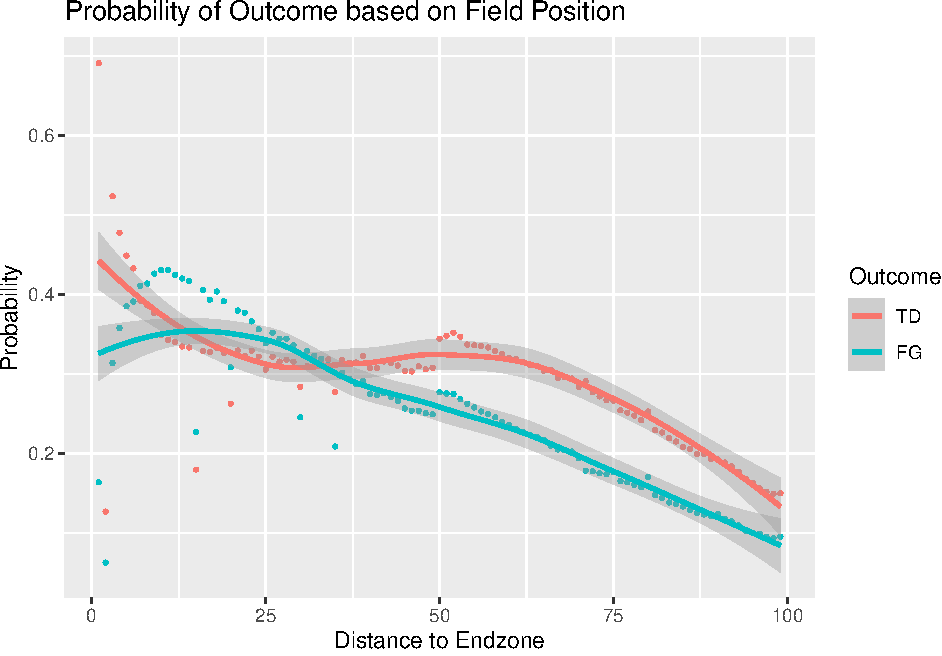
\includegraphics{22-isaac_files/figure-latex/unnamed-chunk-11-1.pdf} Q:
Why does the probability of scoring a field goal get lower as a team is
within 10 yards of the endzone?

A: When a team is close to the endzone, they probability of scoring a
touchdown goes way up so teams are less likely to attempt field goals
since the expected value of attempting a touchdown is higher than the
expected value of attempting a field goal.

\hypertarget{offensive-epa-vs-defensive-epa}{%
\paragraph{Offensive EPA vs Defensive
EPA}\label{offensive-epa-vs-defensive-epa}}

On any given football play, a team has an expected point value (from the
current drive) before the play and an expected point value after the
play. The difference between these expected values, is the change in
expected points that resulted from the play. We can look at each teams
defensive EPA and offensive EPA for the 2021 season.

\begin{Shaded}
\begin{Highlighting}[]
\CommentTok{# read in pbp data}
\NormalTok{pbp=}\KeywordTok{read.csv}\NormalTok{(}\StringTok{'~/Google Drive/My Drive/Sports Analytics/SportsAnalyticsBook/data/nfl_pbp_2021.gz'}\NormalTok{)}
\NormalTok{pbp <-}\StringTok{ }\KeywordTok{select}\NormalTok{(pbp, }\KeywordTok{c}\NormalTok{(}\StringTok{'posteam'}\NormalTok{,}\StringTok{'epa'}\NormalTok{,}\StringTok{'yards_gained'}\NormalTok{,}\StringTok{'defteam'}\NormalTok{))}

\CommentTok{# get offensive epa and epa per play}
\NormalTok{off_df <-}\StringTok{ }\NormalTok{pbp }\OperatorTok
\StringTok{  }\KeywordTok{group_by}\NormalTok{(posteam) }\OperatorTok
\StringTok{  }\KeywordTok{summarise}\NormalTok{(}\DataTypeTok{off_epa =} \KeywordTok{sum}\NormalTok{(epa),}
            \DataTypeTok{off_plays =} \KeywordTok{n}\NormalTok{(),}
            \DataTypeTok{off_epp =}\NormalTok{ off_epa}\OperatorTok{/}\NormalTok{off_plays,}
            \DataTypeTok{.groups=}\StringTok{'drop'}\NormalTok{)}

\CommentTok{# get defensive epa and epa per play}
\NormalTok{def_df <-}\StringTok{ }\NormalTok{pbp }\OperatorTok
\StringTok{  }\KeywordTok{group_by}\NormalTok{(defteam) }\OperatorTok
\StringTok{  }\KeywordTok{summarise}\NormalTok{(}\DataTypeTok{def_epa =} \KeywordTok{sum}\NormalTok{(epa),}
            \DataTypeTok{def_plays =} \KeywordTok{n}\NormalTok{(),}
            \DataTypeTok{def_epp =}\NormalTok{ def_epa}\OperatorTok{/}\NormalTok{def_plays,}
            \DataTypeTok{.groups=}\StringTok{'drop'}\NormalTok{)}
\CommentTok{# merge dataframes}
\KeywordTok{names}\NormalTok{(off_df)[}\KeywordTok{names}\NormalTok{(off_df) }\OperatorTok{==}\StringTok{ 'posteam'}\NormalTok{] <-}\StringTok{ 'team'}
\KeywordTok{names}\NormalTok{(def_df)[}\KeywordTok{names}\NormalTok{(def_df) }\OperatorTok{==}\StringTok{ 'defteam'}\NormalTok{] <-}\StringTok{ 'team'}
\NormalTok{epa_df <-}\StringTok{ }\KeywordTok{merge}\NormalTok{(off_df,def_df,}\DataTypeTok{by=}\StringTok{'team'}\NormalTok{)}
\NormalTok{epa_df <-}\StringTok{ }\KeywordTok{na.omit}\NormalTok{(epa_df)}

\CommentTok{# plot}
\KeywordTok{ggplot}\NormalTok{(epa_df,}\KeywordTok{aes}\NormalTok{(}\DataTypeTok{x=}\NormalTok{off_epp,}\DataTypeTok{y=}\NormalTok{def_epp, }\DataTypeTok{label=}\NormalTok{team))}\OperatorTok{+}\KeywordTok{geom_point}\NormalTok{()}\OperatorTok{+}\KeywordTok{geom_hline}\NormalTok{(}\DataTypeTok{yintercept=}\DecValTok{0}\NormalTok{)}\OperatorTok{+}\KeywordTok{geom_vline}\NormalTok{(}\DataTypeTok{xintercept=}\DecValTok{0}\NormalTok{)}\OperatorTok{+}\KeywordTok{geom_label}\NormalTok{(}\KeywordTok{aes}\NormalTok{(}\DataTypeTok{label =}\NormalTok{ team))}\OperatorTok{+}\KeywordTok{xlab}\NormalTok{(}\StringTok{'Offensive EPA per Play'}\NormalTok{)}\OperatorTok{+}\KeywordTok{ylab}\NormalTok{(}\StringTok{'Defensive EPA per Play'}\NormalTok{)}
\end{Highlighting}
\end{Shaded}

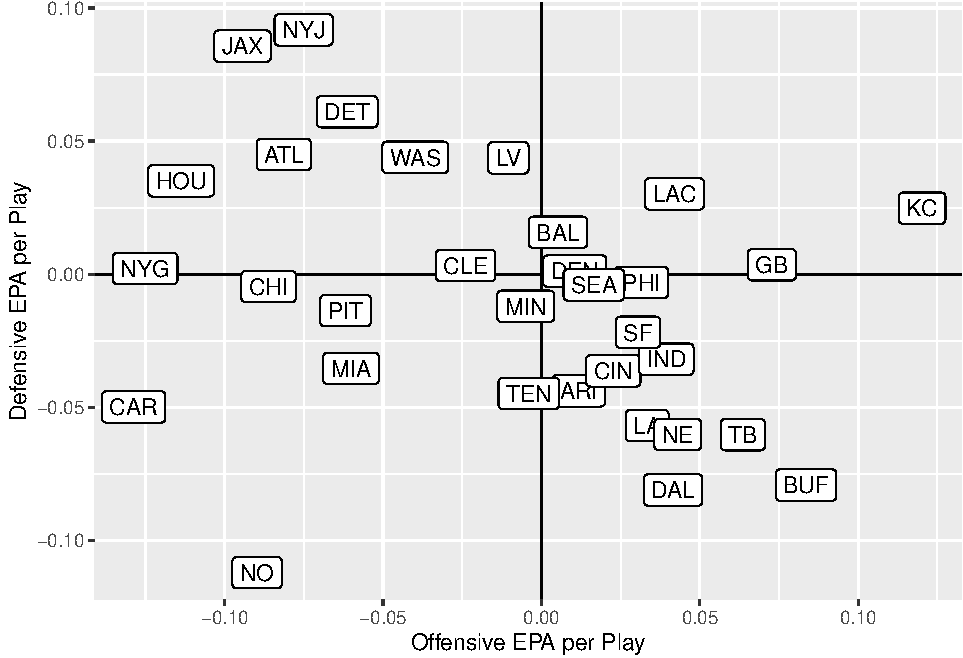
\includegraphics{22-isaac_files/figure-latex/unnamed-chunk-12-1.pdf}

\hypertarget{football-sample-space-probability}{%
\paragraph{Football Sample Space
(Probability)}\label{football-sample-space-probability}}

A sample space contains all possible outcomes. An american football game
can either end with a win (W), loss (L) or a tie (T) which means our
sample space is \(\Omega = \{W,L,T \}\) and an event, \(E\) would be one
of the possible outcomes. If a team wins the game, the event for that
game would be \(E=\{W \}\) or if we want the event of the 2021 CSU
football season, it would be
\(E=\{ L, L, W, L, W, W, L, L, L, L, L, L \}\).

\begin{center}\rule{0.5\linewidth}{\linethickness}\end{center}

\hypertarget{gambling}{%
\subsection{Gambling}\label{gambling}}

\hypertarget{sports-betting-bankroll-management}{%
\subsubsection{Sports Betting Bankroll
Management}\label{sports-betting-bankroll-management}}

To prevent problematic gambling many people use bankrolls, or money set
aside with the sole purpose of gambling. It is often suggested that
people partaking in sports betting set aside an amount they are
comfortable gambling with and betting 1-5\% of that per play, especially
considering minimum bets for online sportsbooks are often less than \$1.
One of the big risks in gambling is chasing losses so a popular strategy
is called flat betting, where you bet the same amount on every game to
help minimize losses. In addition, parlays can have incredibly
attractive payoffs but high reward comes with high risk so it can be
quite difficult to find long term profit.

\hypertarget{hold-percentagebreaking-even}{%
\subsubsection{Hold Percentage/Breaking
Even}\label{hold-percentagebreaking-even}}

In a perfect world, if a baseball game has probability 0.5 of either
team winning, the odds would be +100 (or -100), 50\% of bettors would be
on one side, 50\% on the other, and at the end of the game half of the
bettors would double their money and half of them would lose their
money. Unfortunately, this would mean that the casinos make no money so
to combat this they introduce whats called a hold percentage.
Essentially sportsbooks will give you slightly worse odds on bets in
order to make money. In this example, when both sides have probability
0.5, the offered lines may both be -110 that way when one team wins,
half the bettors win slightly less than double the money (bet 110
dollars to win 100) and the sportsbook collects the rest. As a result,
winning percentages have to be higher than expected to show a profit.
For -110 odds (the Vegas equivalent of probability = 0.5), a bettor must
win at a rate of 52.23\% of the time in order to show a profit.
Similarly you can convert any American odds into implied probability to
get a breakeven percentage, since if you have a win rate higher than the
implied probability, the expected value of your bet is positive.

Q: The given odds for the Avs to win the 2022 Stanley Cup are +500 and
you've concluded that the bet has a 15\% chance of happening. Is it
worth making this bet?

A: The implied probability on a +500 bet is 16.66\%, therefore if the
bet has a 15\% chance of happening, it is not a good bet as the expected
value is negative but lets look at a simulation.

\begin{Shaded}
\begin{Highlighting}[]
\CommentTok{# lets say we start with $1 and we want to bet $1}
\NormalTok{dollars =}\StringTok{ }\DecValTok{1}
\KeywordTok{set.seed}\NormalTok{(}\DecValTok{1}\NormalTok{)}
\CommentTok{# we want to simulate the bet 100,000 times}
\NormalTok{n.sims <-}\StringTok{ }\DecValTok{100000}
\ControlFlowTok{for}\NormalTok{(i }\ControlFlowTok{in} \DecValTok{1}\OperatorTok{:}\NormalTok{n.sims)\{}
\CommentTok{# Simulate whether the Avs win based on our probability of 15%}
\NormalTok{  win <-}\StringTok{ }\KeywordTok{sum}\NormalTok{(}\KeywordTok{rbinom}\NormalTok{(}\DecValTok{1}\NormalTok{,}\DecValTok{1}\NormalTok{,}\FloatTok{0.15}\NormalTok{))}
  \CommentTok{# change our dollar amount based off the odds}
  \ControlFlowTok{if}\NormalTok{(win }\OperatorTok{==}\StringTok{ }\DecValTok{1}\NormalTok{)\{}
\NormalTok{    dollars =}\StringTok{ }\NormalTok{dollars }\OperatorTok{+}\StringTok{ }\DecValTok{5}
\NormalTok{  \}}
  \ControlFlowTok{if}\NormalTok{(win }\OperatorTok{==}\StringTok{ }\DecValTok{0}\NormalTok{)\{}
\NormalTok{    dollars =}\StringTok{ }\NormalTok{dollars }\OperatorTok{-}\StringTok{ }\DecValTok{1}
\NormalTok{  \}}
\NormalTok{\}}
\KeywordTok{print}\NormalTok{(dollars)}
\end{Highlighting}
\end{Shaded}

\begin{verbatim}
## [1] -9573
\end{verbatim}

After 100,000 bets, we would be down 9,573 dollars just off of 1 dollar
bets.

\hypertarget{gamblers-fallacy}{%
\subsubsection{Gamblers Fallacy}\label{gamblers-fallacy}}

The Gambler's Fallacy is the common misbelief that if independent events
fail to happen, theyre more likely to happen in the future. For example,
say we are playing Roulette and betting on whether the ball lands on
black or red. Theres roughly a 50\% chance of either outcome, yet if we
somehow get 10 reds in a row, the natural inclination is to assume a
black is ``due'' and must come soon. However, both outcomes still have
just a 50\% chance of happening regardless of the history. This can be
seen in the sports world as well, especially when talking about
something like the `hot hand' in basketball or hitting streaks in
baseball, although sports does differ from conventional gambling as
recent performance in sports can be useful for predictive purposes.

\hypertarget{kelly-criterion}{%
\subsubsection{Kelly Criterion}\label{kelly-criterion}}

While flat betting is a common and effective bet sizing strategy, a more
advanced technique is called the Kelly Criterion. The Kelly Criterion
adjusts each bet size to the specific bet based on bankroll size, given
odds, and the predicted probability that the bettor gives the outcome.
The formula for calculating the bet size is \(f=p-\frac{1-p}{b}\) where
\(f\) is the fraction of your current bankroll you should wager, \(p\)
is the probability the bettor gives themselves of winning the bet, and
\(b\) is the proportion of the bet you win back (+200 odds pays 2 to 1
therefore the proportion is 2.0). This is certainly more complicated
than flat betting (especially in large volumes), but it has been proven
to provide theoretically optimal bet sizes.

\hypertarget{unfinished-ideas-for-both-classes}{%
\subsection{UNFINISHED IDEAS (for both
classes)}\label{unfinished-ideas-for-both-classes}}

\hypertarget{football}{%
\subsubsection{Football}\label{football}}

\hypertarget{average-expected-points-by-field-position}{%
\paragraph{Average Expected Points by Field
Position}\label{average-expected-points-by-field-position}}

\hypertarget{should-you-go-for-it-on-4th-down}{%
\paragraph{Should you go for it on 4th
down?}\label{should-you-go-for-it-on-4th-down}}

\hypertarget{tennis-1}{%
\subsubsection{Tennis}\label{tennis-1}}

\hypertarget{difference-of-means-nadal-on-clay-vs-other-surfaces}{%
\paragraph{Difference of means Nadal on clay vs other
surfaces}\label{difference-of-means-nadal-on-clay-vs-other-surfaces}}

\hypertarget{linear-regression-contrast-nadal-on-clay-vs-other-surfaces}{%
\paragraph{Linear Regression contrast nadal on clay vs other
surfaces}\label{linear-regression-contrast-nadal-on-clay-vs-other-surfaces}}

\hypertarget{basketball}{%
\subsubsection{Basketball}\label{basketball}}

\hypertarget{difference-in-means-clutch-basketball-moments-high-leverage-situation-vs-low-leverage-situation}{%
\paragraph{Difference in means clutch basketball moments (high leverage
situation vs low leverage
situation)}\label{difference-in-means-clutch-basketball-moments-high-leverage-situation-vs-low-leverage-situation}}

\#Baseball

\hypertarget{random-forest-pitch-classification}{%
\paragraph{Random Forest pitch
classification}\label{random-forest-pitch-classification}}

\hypertarget{scrape-daily-lineups-from-baseballpress.com-and-get-summary-statistics-from-baseballr-or-other-package}{%
\paragraph{Scrape daily lineups from baseballpress.com and get summary
statistics from baseballr or other
package}\label{scrape-daily-lineups-from-baseballpress.com-and-get-summary-statistics-from-baseballr-or-other-package}}

\hypertarget{how-relevant-is-1st-inning-pitching-performance-to-the-rest-of-the-games-performance}{%
\paragraph{How relevant is 1st inning pitching performance to the rest
of the games
performance?}\label{how-relevant-is-1st-inning-pitching-performance-to-the-rest-of-the-games-performance}}

\hypertarget{comparing-difference-of-means-of-lefty-pitchers-vs-righties}{%
\paragraph{Comparing difference of means of lefty pitchers vs
righties}\label{comparing-difference-of-means-of-lefty-pitchers-vs-righties}}

\hypertarget{hockey}{%
\subsubsection{Hockey}\label{hockey}}

\hypertarget{difference-in-means-scoring-between-2nd-and-3rd-period}{%
\paragraph{Difference in means scoring between 2nd and 3rd
period}\label{difference-in-means-scoring-between-2nd-and-3rd-period}}

\hypertarget{misc}{%
\subsubsection{Misc}\label{misc}}

\hypertarget{assignemnt-idea-where-the-main-purpose-is-creating-interesting-visualizations-from-a-dataset-since-conveying-statistical-information-to-others-is-often-as-important-as-understanding-it-yourself}{%
\paragraph{Assignemnt idea where the main purpose is creating
interesting visualizations from a dataset since conveying statistical
information to others is often as important as understanding it
yourself}\label{assignemnt-idea-where-the-main-purpose-is-creating-interesting-visualizations-from-a-dataset-since-conveying-statistical-information-to-others-is-often-as-important-as-understanding-it-yourself}}


\end{document}
